\chapter{膜运输与蛋白质分选}\label{ch:b3:membrane-traffic}

胰腺细胞每分钟制造约一千万个消化酶分子，
将其装入颗粒，并在肠道信号的作用下释放到导管中，
而从不让一个胰蛋白酶分子漏入自身的细胞质。
肝细胞从血液中摄取胆固醇，方式是整颗吞入携带它的颗粒，
速率每分钟可达数千个；
随后每个受体都被送回表面，供下一轮使用。
新合成的蛋白质若要前往线粒体、细胞核、\omterm{def:b3:membrane-traffic:endocytosis}{溶酶体}、
膜或胞外，需在十余个区室之间找到正确的“地址”，
其差错率足以让邮政部门汗颜。
本章讨论的正是这种分选：蛋白质上的信号、读取信号的机器、
在区室之间运载膜与货物的囊泡、塑造囊泡形态的\omterm{def:b3:membrane-traffic:coats}{衣被}，
使囊泡与正确靶标融合的蛋白质，
以及分泌（向外）与胞吞（向内）
这两种双向运输，
真核细胞一生中每一秒都在进行这些运输。

\section{信号与地址}

\begin{definition}[分选信号]\label{def:b3:membrane-traffic:signals}
\index{分选信号}\index{信号肽}\index{核定位信号}\index{前导序列}
\emph{分选信号}是蛋白质的一段序列，或其上的一种修饰，
由受体识别后将该蛋白质递送至某一区室。
\emph{信号肽}是位于氨基端、长 \numrange{15}{30} 个残基、
带有疏水核心的一段序列，在蛋白质合成时引导其进入内质网；
此后默认途径经高尔基体通向质膜或胞外，
另有信号使蛋白质转向\omterm{def:b3:membrane-traffic:endocytosis}{溶酶体}（一种磷酸化糖），
或经内质网返回（羧基端序列 KDEL）。
\emph{核定位信号}是一段短的碱性序列，如 PKKKRKV，
可被核转运蛋白（importin）结合，并携带折叠状态的蛋白质穿过核孔；
线粒体\emph{前导序列}是一段长 \numrange{20}{50} 个残基的两亲性螺旋，
由外膜上的受体识别，并以未折叠状态穿过两层膜上的转位酶；
过氧化物酶体的酶以 SKL 结尾。
不含以上任何信号的蛋白质留在细胞质中。
每种信号都以同样方式被发现：删除该信号，
蛋白质即留在细胞质中；
将该信号接到细胞质蛋白上，
则该蛋白质被送入相应区室。
\end{definition}

\begin{proof}[证据]
Blobel 和 Dobberstein（1975）在无细胞体系中翻译了抗体轻链的信使 RNA。
无膜时，产物比分泌蛋白长约二十个残基；
若在翻译\emph{过程中}加入内质网碎片，
产物则具有分泌蛋白的大小，并能抵抗外加蛋白酶的降解——
说明它位于囊泡内部；
而翻译结束后再加入膜则毫无作用。
多出的氨基端片段即\omterm{def:b3:membrane-traffic:signals}{信号肽}，它是进入内质网所必需的，
在内质网内被切除，且仅在肽链合成过程中起作用：
这就是\emph{信号假说}，
其在每个细节上都得到证实，
即在受体（信号识别颗粒，Walter 和 Blobel，1981）
与通道（Sec61）被纯化之后。
\end{proof}

\begin{omfigure}
\begin{tikzpicture}[every node/.style={font=\scriptsize}, >=stealth]
  % ER membrane
  \fill[omDef!15] (0,0) rectangle (12,-1.6);
  \draw[very thick, omDef] (0,0) -- (12,0); \draw[very thick, omDef] (0,-0.35) -- (12,-0.35);
  \node[right, omDef!70!black] at (0.1,-1.3) {内质网腔};
  \node[right] at (0.1,2.9) {细胞质};
  % stage 1: ribosome with emerging signal peptide + SRP
  \draw[thick, fill=gray!25] (1.4,1.6) circle (0.5); \draw[thick, fill=gray!25] (1.4,0.95) ellipse (0.62 and 0.3);
  \draw[very thick, omThm] (1.4,0.65) -- (1.4,0.2) -- (1.9,0.1);
  \draw[thick, fill=omProp!40] (2.1,0.35) ellipse (0.35 and 0.2); \node[above right] at (2.2,0.5) {SRP};
  \node[below, align=center] at (1.7,-1.7) {1. 信号肽露出；\\SRP 结合，翻译暂停};
  % stage 2: docking at SRP receptor and translocon
  \draw[->, thick] (3.2,1.2) -- (4.2,1.2);
  \draw[thick, fill=gray!25] (5.6,1.75) circle (0.5); \draw[thick, fill=gray!25] (5.6,1.1) ellipse (0.62 and 0.3);
  \draw[thick, fill=omMeth!40] (5.2,0.0) rectangle (5.45,-0.35); \draw[thick, fill=omMeth!40] (5.75,0.0) rectangle (6.0,-0.35);
  \node[below, align=center] at (5.9,-1.7) {2. SRP 受体将其对接于 \\Sec61 上，SRP 离开};
  \draw[very thick, omThm] (5.6,0.8) -- (5.6,-0.2);
  \draw[thick, fill=omProp!40] (4.7,0.15) ellipse (0.3 and 0.18); \node[above] at (4.7,0.33) {SRP 受体};
  % stage 3: translocation, cleavage, glycosylation
  \draw[->, thick] (7.2,1.2) -- (8.2,1.2);
  \draw[thick, fill=gray!25] (9.6,1.75) circle (0.5); \draw[thick, fill=gray!25] (9.6,1.1) ellipse (0.62 and 0.3);
  \draw[thick, fill=omMeth!40] (9.2,0.0) rectangle (9.45,-0.35); \draw[thick, fill=omMeth!40] (9.75,0.0) rectangle (10.0,-0.35);
  \draw[very thick, omThm] (9.6,0.8) -- (9.6,-0.5) .. controls (9.6,-1.0) and (10.3,-1.1) .. (10.6,-0.7);
  \draw[omThm, thick] (10.9,-0.9) -- (11.2,-0.9); \node[right, font=\tiny] at (11.0,-1.15) {信号切除};
  \fill[omExo] (10.3,-1.0) circle (0.07); \fill[omExo] (10.45,-1.12) circle (0.07); \node[below, font=\tiny] at (10.2,-1.15) {糖类};
  \node[below, align=center] at (10.0,-1.7) {3. 肽链边合成边穿膜；\\信号切除，并加上糖类};
\end{tikzpicture}

{\small 信号假说。新生肽链起始处的\omterm{def:b3:membrane-traffic:signals}{信号肽}
被信号识别颗粒结合，后者使翻译暂停，
并将核糖体对接到 Sec61 通道上；随后肽链
边合成边穿过膜，\omterm{def:b3:membrane-traffic:signals}{信号肽}在腔内被切除，
并加上糖类。}
\end{omfigure}

\begin{proposition}[膜蛋白与拓扑结构]\label{prop:b3:membrane-traffic:topology}
\index{停止转移序列}\index{膜拓扑结构}
在被转位的肽链中部，一段约二十个残基的疏水序列
充当\emph{停止转移}序列：通道侧向开放，
将其释放进入脂双层，形成一段跨膜螺旋；
已转位部分位于腔内，其余部分则进入细胞质。
第二段此类序列可重新启动转位，
含 $n$ 个交替信号的蛋白质
则带有 $n$ 段跨膜螺旋。内质网中所设定的方向
永不改变：朝向内质网腔的一侧，
在此之后的高尔基体腔及每个囊泡的腔内都朝向同一侧，并在与质\omterm{def:b3:membrane-traffic:fusion}{膜融合}后朝向细胞的\emph{外侧}。
因此，仅在腔内添加的糖类
总是位于表面蛋白的胞外面，
故受体的拓扑结构，
可由其糖基化位点的位置读出。
\end{proposition}

\begin{method}[脉冲–追踪]\label{met:b3:membrane-traffic:pulse-chase}
\index{脉冲–追踪}\index{放射自显影}
要追踪新合成的分子群体在细胞内的去向：(1)
用放射性或其他标记的前体短暂处理细胞（即\emph{脉冲}，几分钟）；
蛋白质常用的前体为氚标记的亮氨酸。(2) 随后换用过量未标记的前体（即\emph{追踪}），
使新的标记不再掺入；(3) 每隔一定时间取样并固定细胞，
通过\omterm{met:b3:membrane-traffic:pulse-chase}{放射自显影}在电镜照片中定位标记，
或分离各区室后计数；(4) 以各区室中标记所占比例对时间作图。
各区室中标记充盈与消失的先后次序即为运输途径，
时间则给出各区室中的停留时间。
帕拉德实验室（1960 年代）将该方法用于胰腺腺泡细胞，
发现标记在粗面内质网中出现的时间为
\qty{3}{min}，在高尔基体中为 \qty{20}{min}，
在浓缩液泡与颗粒中为 \qty{40}{min}，
并于一小时后进入导管，且在信号作用下释放；
分泌途径由此按时间顺序展开。
\end{method}

\begin{theorem}[连续区室与脉冲–追踪曲线]\label{thm:b3:membrane-traffic:pulse-chase}
\index{区室模型}
设带标记的蛋白质脉冲由区室 $A$ 进入 $B$，
一级速率为 $k_{1}$；再由 $B$ 进入 $C$，速率为 $k_{2}$，$C$ 保留之。
标记全部位于 $A$ 中，取 $t = 0$：
\[
A(t) = e^{-k_{1}t},\qquad
B(t) = \frac{k_{1}}{k_{2} - k_{1}}\bigl(e^{-k_{1}t} - e^{-k_{2}t}\bigr),
\qquad
C(t) = 1 - A - B,
\]
且 $B$ 中的标记在 $t^{*} = \ln(k_{2}/k_{1})/(k_{2} - k_{1})$ 时达到峰值。
在 $A$ 中的平均停留时间为 $1/k_{1}$，在 $B$ 中为 $1/k_{2}$，
与两速率的大小次序无关。
\end{theorem}
\begin{proof}
由 $\mathrm{d}A/\mathrm{d}t = -k_{1}A$ 得指数函数。对 $B$，
$\mathrm{d}B/\mathrm{d}t = k_{1}A - k_{2}B = k_{1}e^{-k_{1}t} - k_{2}B$;
试取 $B = \beta(e^{-k_{1}t} - e^{-k_{2}t})$，其导数为
$\beta(-k_{1}e^{-k_{1}t} + k_{2}e^{-k_{2}t})$，且 $-k_{2}B = \beta(-k_{2}
e^{-k_{1}t} + k_{2}e^{-k_{2}t})$，故方程要求 $\beta(k_{2}
- k_{1})e^{-k_{1}t} = k_{1}e^{-k_{1}t}$，$\beta = k_{1}/(k_{2} -
k_{1})$，且 $B(0) = 0$ 满足初始条件。令 $\mathrm{d}B/\mathrm{d}t =
0$：$k_{1}e^{-k_{1}t} = k_{2}e^{-k_{2}t}$，由此得 $t^{*}$。
一个分子在以速率 $k$ 离开的区室中的平均停留时间为 $\int_{0}^{
\infty} t\,k e^{-kt}\,\mathrm{d}t = 1/k$。
\end{proof}

\begin{example}[帕拉德细胞的数值示例]\label{ex:b3:membrane-traffic:palade}
取 $k_{1} = \qty{0.1}{min^{-1}}$（内质网中停留十分钟）和
$k_{2} = \qty{0.05}{min^{-1}}$（高尔基体中停留二十分钟）。高尔基体中的标记在
$t^{*} = \ln 2/0.05 = \qty{13.9}{min}$ 时达峰，此时 $B = 2(e^{-1.39} -
e^{-0.69}) = 2(0.25 - 0.50)\cdot(-1) = 0.50$，即一半标记。在
\qty{40}{min}时，$A = 0.018$，$B = 2(0.018 - 0.135) \to 0.23$，$C = 0.75$：
四分之三的蛋白质已到达颗粒。帕拉德实验室观测到的
曲线即呈此形态，而拟合它们正是
最初测定停留时间的办法。
\end{example}

\begin{omfigure}
\begin{tikzpicture}
\begin{axis}[
  width=0.7\linewidth, height=5.6cm,
  axis x line=bottom, axis y line=left,
  xmin=0, xmax=80, ymin=0, ymax=1.05,
  xlabel={脉冲后分钟数}, ylabel={标记比例},
  xlabel style={font=\small, at={(axis description cs:0.5,-0.12)}, anchor=north},
  ylabel style={font=\small},
  tick label style={font=\small}, xtick={0,20,40,60,80}, ytick={0,0.5,1},
  clip=false,
]
\addplot[very thick, omDef, domain=0:80, samples=80] {exp(-0.1*x)};
\addplot[very thick, omProp, domain=0:80, samples=80] {2*(exp(-0.05*x)-exp(-0.1*x))};
\addplot[very thick, omMeth!70!black, domain=0:80, samples=80] {1-exp(-0.1*x)-2*(exp(-0.05*x)-exp(-0.1*x))};
\node[font=\scriptsize, omDef, anchor=south west] at (axis cs:4,0.62) {内质网，$A$};
\node[font=\scriptsize, omProp, anchor=south] at (axis cs:14,0.53) {高尔基体，$B$};
\node[font=\scriptsize, omMeth!70!black, anchor=north west] at (axis cs:45,0.72) {颗粒，$C$};
\end{axis}
\end{tikzpicture}

{\small 双速率模型的\omterm{met:b3:membrane-traffic:pulse-chase}{脉冲–追踪}曲线，取 $k_{1} =
\qty{0.1}{min^{-1}}$ 和 $k_{2} = \qty{0.05}{min^{-1}}$：标记从
内质网中按指数衰减，经高尔基体后于
\qty{14}{min}时达峰，并在颗粒中积累。}
\end{omfigure}

\section{内质网：折叠、糖链与质量控制}

\begin{definition}[N-糖基化与质量控制]\label{def:b3:membrane-traffic:glycosylation}
\index{N-糖基化}\index{钙连蛋白循环}\index{内质网相关降解}\index{未折叠蛋白反应}
肽链进入内腔时，一个预先\omterm{def:b3:genomics:assembly}{组装}好的寡糖，
（含十四个糖：两个 N-乙酰葡糖胺、九个甘露糖、三个
葡萄糖），由脂质载体转移到
序列 Asn-X-Ser/Thr 中的天冬酰胺上——\emph{N-糖基化}。三个葡萄糖
随后逐一修剪，修剪过程即为折叠“计时器”：
仍保留一个葡萄糖的蛋白质由\omterm{def:b3:structural-biology:chaperones}{分子伴侣}钙连蛋白结合；
末端葡萄糖已被去除而尚未折叠的蛋白质，
会被一种能识别暴露的
疏水斑块的酶重新糖基化，并回到钙连蛋白——即\emph{钙连蛋白
循环}。反复失效的蛋白质被拉回细胞溶胶，
泛素化并被蛋白酶体降解：\emph{内质网相关
降解}（ERAD）。当未折叠蛋白的积累快于
它们被折叠或降解的速度时，内质网膜上的传感器
启动\emph{未折叠蛋白反应}：翻译减慢，
\omterm{def:b3:structural-biology:chaperones}{分子伴侣}基因被诱导表达，内质网扩张，若应激
持续，则细胞被杀死。囊性纤维化最常见的突变
（CFTR 中的 $\Delta$F508）使通道本可工作，却折叠过慢，
被 ERAD 捕获，永不能到达表面；能助其折叠的药物
现已成为一种治疗手段。
\end{definition}

\begin{omfigure}
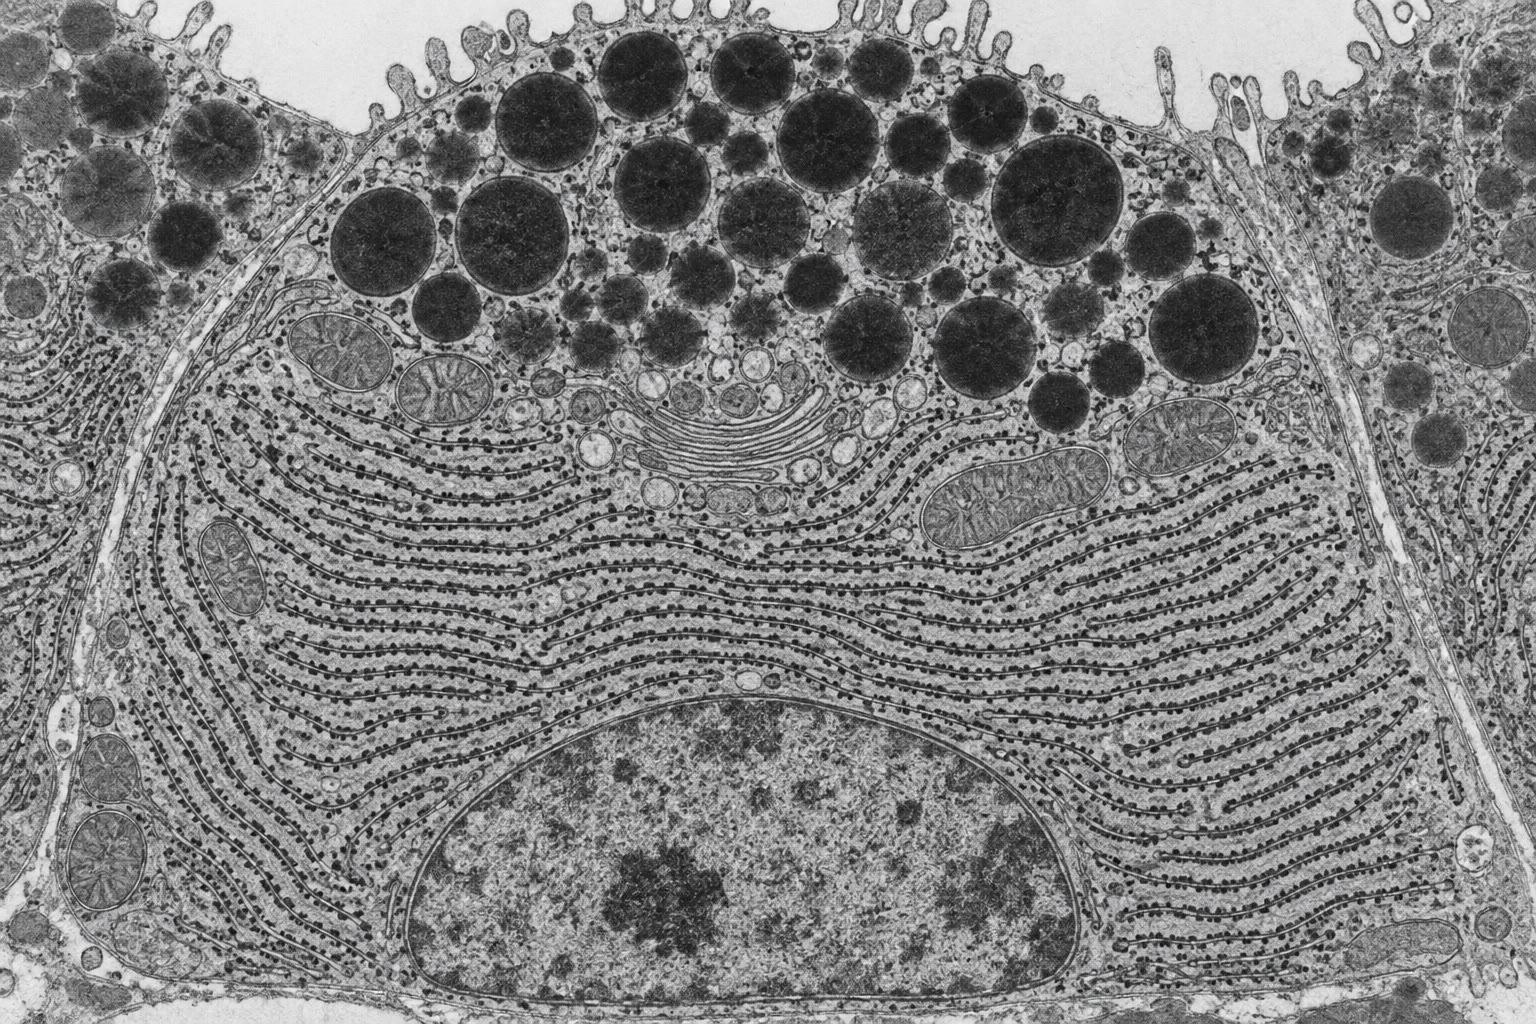
\includegraphics[width=0.56\linewidth]{images/book5/ai/b5-08-pancreas-acinar.jpg}

{\small 胰腺腺泡细胞的电镜照片：堆叠的
附有核糖体的粗面内质网充满基部，
高尔基体位于细胞核上方，致密的
消化酶分泌颗粒堆积于顶端表面下方，等待
信号。}
\end{omfigure}

\section{囊泡：出芽、靶向与融合}

\begin{definition}[衣被与囊泡出芽]\label{def:b3:membrane-traffic:coats}
\index{有被囊泡}\index{COPII}\index{COPI}\index{网格蛋白}\index{小 GTP 酶}
运输囊泡由一层蛋白质\emph{衣被}塑造，该衣被装配于
膜的胞质面上，使膜弯曲成芽状突起，
直径为 \qtyrange{60}{100}{nm} 的芽体，通过跨膜受体收集货物，
并在囊泡夹断后脱落。三种衣被
服务于主要运输途径：\emph{COPII} 负责离开内质网、
前往高尔基体的囊泡，\emph{COPI} 负责从高尔基体
回到内质网及高尔基体膜囊之间的回流运输，以及\emph{网格蛋白}——一
种三足蛋白，可聚合成由六边形和
五边形组成的笼——负责由反面高尔基体去往\omterm{def:b3:membrane-traffic:endocytosis}{内体}的囊泡，以及
质膜处的胞吞作用，衔接蛋白将笼与
被内化的受体相连。每种衣被由
一种\emph{小 GTP 酶}招募（COPII 为 Sar1，COPI 与网格蛋白为 Arf1），
该酶以 GTP 结合态插入膜中，出芽后水解 GTP，
使衣被脱落。回收信号使各区室保持区分：
携带 KDEL 的内质网蛋白若逃逸，在高尔基体中被受体结合，
并由 COPI 囊泡运回。
\end{definition}

\begin{omfigure}
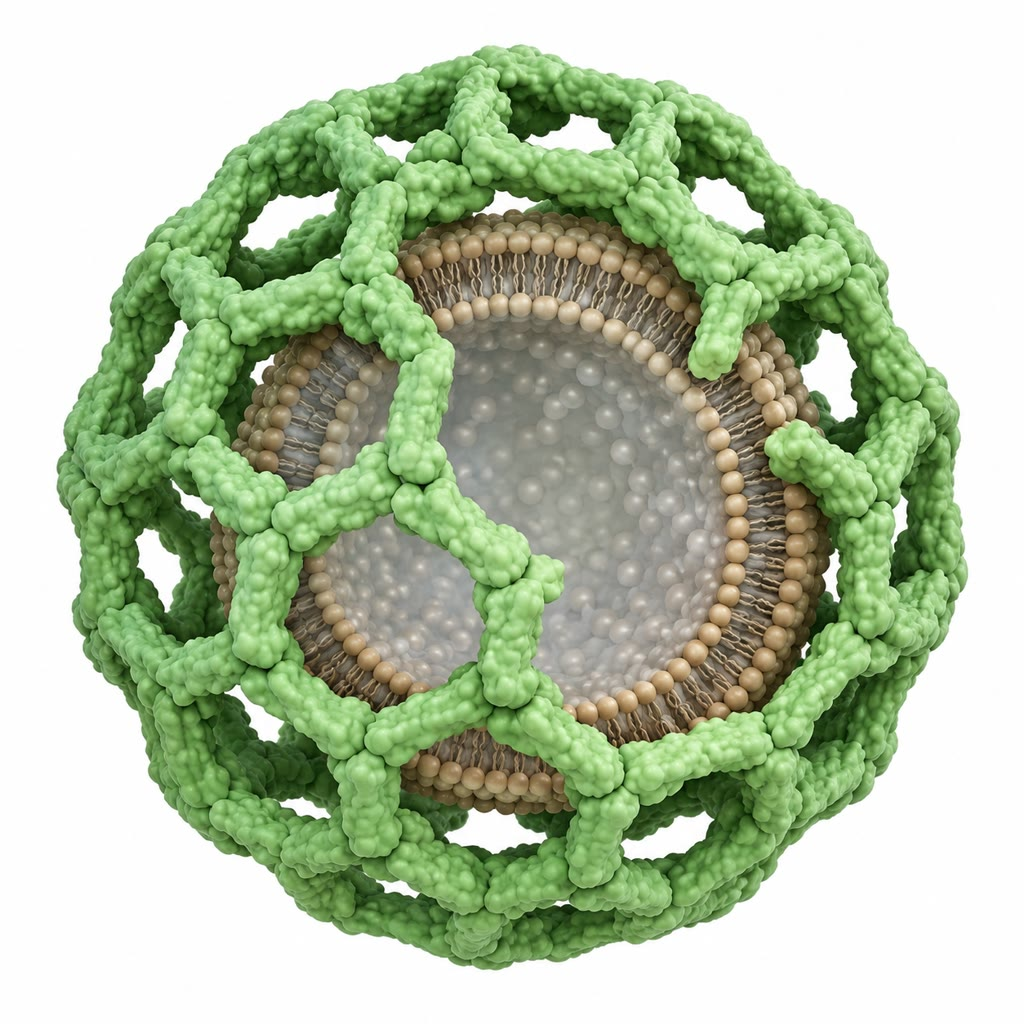
\includegraphics[width=0.36\linewidth]{images/book5/ai/b5-08-clathrin-cage.jpg}\hspace{0.04\linewidth}
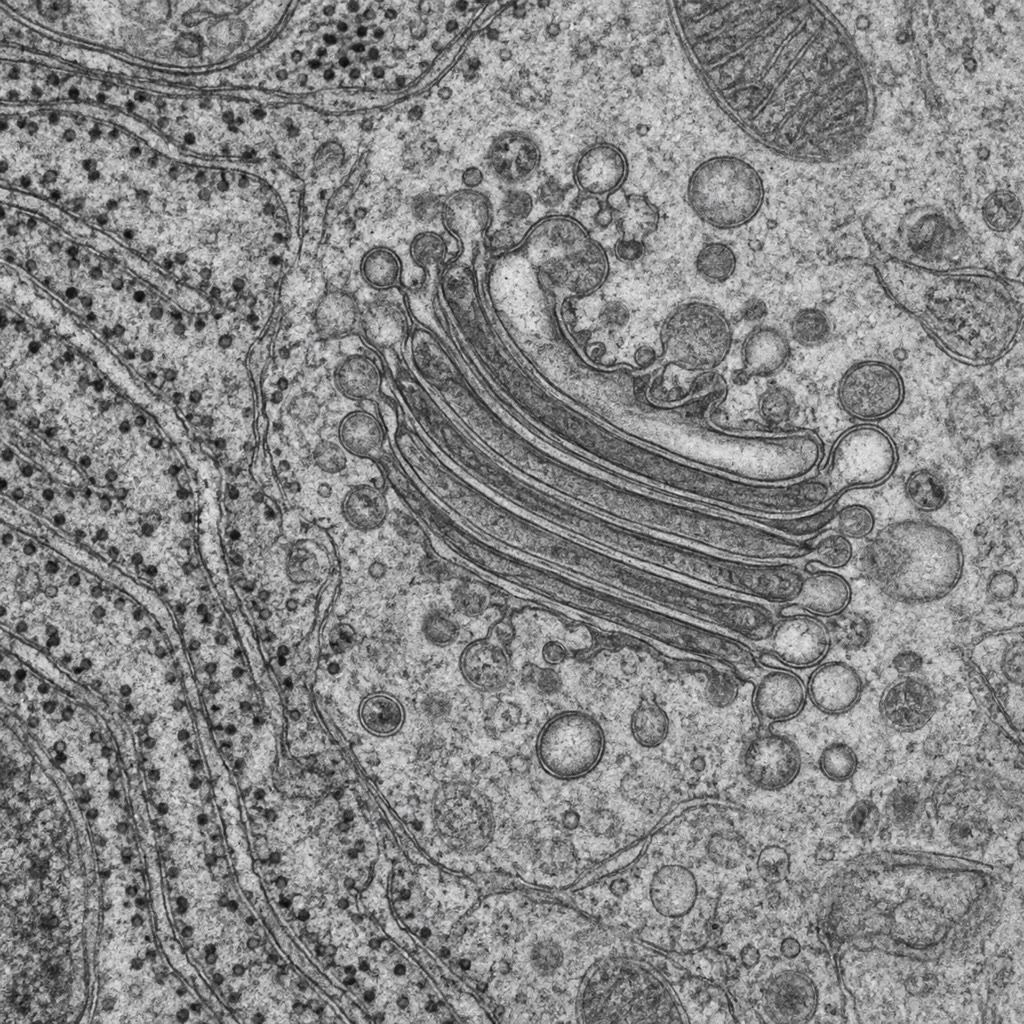
\includegraphics[width=0.36\linewidth]{images/book5/ai/b5-08-golgi-tem.jpg}

{\small 左：\omterm{def:b3:membrane-traffic:coats}{网格蛋白}笼，由三足单元组成的多面体晶格，塑造出胞吞囊泡
（切开以露出内部的膜）。右：
电子显微镜下的高尔基体堆叠，一摞
扁平的囊槽，边缘有囊泡出芽。}
\end{omfigure}

\begin{definition}[靶向与融合]\label{def:b3:membrane-traffic:fusion}
\index{Rab GTP 酶}\index{SNARE}\index{膜融合}\index{突触结合蛋白}
囊泡通过两层识别找到靶标。\emph{Rab
GTP 酶}——人类细胞中约有六十种，各位于一个区室的膜上，
招募长的系绳蛋白，它们捕获携带匹配 Rab 的入站囊泡。
随后 \emph{SNARE} 发挥作用：
囊泡上为 v-SNARE，靶膜上为 t-SNARE，二者都是螺旋蛋白，
锚定于各自的膜中，从远端向膜的方向彼此缠绕，
二者形成的四螺旋束所释放的能量
将两层脂双层拉近直至融合。每一对 SNARE 的配对都具有专一性，
这构成对靶向地址的第二重核验。融合之后，
复合体由 ATP 酶 NSF 拆开，以便重复利用。融合可以设计为推迟，
待信号到来：在神经末梢，SNARE 由 complexin 维持半拉链状态，
直至\emph{突触结合蛋白}与动作电位到达时流入的钙离子结合，
完成拉链闭合，耗时不足一毫秒——
这一神经递质释放过程见于本科二年级
分册。破伤风与肉毒中毒的神经毒素
是切割 SNARE 的蛋白酶。
\end{definition}

\begin{proof}[证据]
诺维克与谢克曼（1980）分离出温度敏感型酵母
突变体，它们在 \qty{37}{\celsius} 下停止分泌，并在其缺陷所阻断的区室中积累蛋白质——
内质网、高尔基体，或堆积在表面下的囊泡；其中
$23$ 个 \emph{sec} 基因界定了各步骤，
克隆后发现它们编码\omterm{def:b3:membrane-traffic:coats}{衣被}、
小 GTP 酶与 \omterm{def:b3:membrane-traffic:fusion}{SNARE}。罗斯曼在试管中重建了高尔基体囊槽间的运输，
所用为纯化的膜、细胞溶胶与 ATP，
并由此纯化出 NSF 与 \omterm{def:b3:membrane-traffic:fusion}{SNARE}；两种途径汇聚于同样的蛋白，
酵母与哺乳动物的运输机器
被证明为同一套机器。
\end{proof}

\begin{omfigure}
\begin{tikzpicture}[every node/.style={font=\scriptsize}, >=stealth]
  % three stages left to right
  \foreach \x/\gap/\lab in {0/1.2/{1. 由 Rab 拴系}, 4.4/0.55/{2. SNARE 拉链式组装}, 8.8/0.0/{3. 融合，释放货物}} {
    % target membrane
    \draw[very thick, omDef] (\x,0) -- (\x+3.4,0); \draw[very thick, omDef] (\x,-0.3) -- (\x+3.4,-0.3);
    \node[below, align=center] at (\x+1.7,-0.45) {\lab};
  }
  % stage 1 vesicle
  \draw[very thick, omProp] (1.7,1.2+0.8) circle (0.8); \draw[very thick, omProp] (1.7,1.2+0.8) circle (0.6);
  \draw[omThm, thick] (1.4,1.25) -- (1.4,0.35); \draw[omThm, thick] (2.0,1.25) -- (2.0,0.35);
  \draw[omMeth!70!black, thick] (1.7,1.2) -- (1.7,0.6); \draw[omMeth!70!black, thick] (1.7,0.6) -- (1.7,0.0);
  \draw[thick, fill=omExo!40] (0.7,0.9) ellipse (0.25 and 0.2); \node[left] at (0.45,0.9) {Rab 蛋白};
  \draw[thick, omExo!70!black] (0.95,0.9) .. controls (1.1,0.5) .. (1.2,0.05); \node[left, font=\tiny] at (0.9,0.4) {系绳};
  \node[right, font=\tiny] at (2.05,0.8) {SNARE 蛋白};
  % stage 2 vesicle closer, helices twisted
  \draw[very thick, omProp] (6.1,0.55+0.8) circle (0.8); \draw[very thick, omProp] (6.1,0.55+0.8) circle (0.6);
  \draw[omThm, very thick] (5.85,0.6) .. controls (6.2,0.5) and (5.9,0.3) .. (6.1,0.05);
  \draw[omMeth!70!black, very thick] (6.35,0.6) .. controls (6.0,0.5) and (6.3,0.3) .. (6.1,0.05);
  \node[right, font=\tiny, align=left] at (6.6,0.35) {四螺旋束 \\将两层膜拉近};
  % stage 3 fused omega shape
  \draw[very thick, omProp] (9.7,0) .. controls (9.7,1.5) and (11.3,1.5) .. (11.3,0);
  \draw[very thick, omProp] (9.9,-0.3) .. controls (9.9,1.1) and (11.1,1.1) .. (11.1,-0.3);
  \foreach \p in {(10.5,-0.9),(10.2,-1.1),(10.8,-1.15)} \fill[omExo] \p circle (0.06);
  \draw[->, omExo, thick] (10.5,0.5) -- (10.5,-0.6);
  \node[right, font=\tiny, align=left] at (11.4,0.8) {稍后由 NSF\\拆开 \\SNARE};
\end{tikzpicture}

{\small 融合分三步。囊泡上的 Rab 与靶膜上的系绳
蛋白使两层膜进入可相互靠近的距离；囊泡与靶膜上的
\omterm{def:b3:membrane-traffic:fusion}{SNARE}（红色与绿色）拉链式缠绕成四螺旋束，
拉动两层脂双层靠拢；二者随后融合，
货物进入靶区室。}
\end{omfigure}

\begin{proposition}[高尔基体]\label{prop:b3:membrane-traffic:golgi}
\index{高尔基体}\index{囊槽成熟}\index{甘露糖-6-磷酸}
高尔基体是由四至八个扁平囊槽堆叠而成的结构，顺面
朝向内质网，反面朝向质膜，每个
囊槽含有一组不同的酶，用于修剪和重建
经过的糖蛋白上的糖链，并添加 O-连接的糖、硫酸基团与
磷酸基团。货物主要通过\emph{\omterm{prop:b3:membrane-traffic:golgi}{囊槽成熟}}推进：新的
囊槽在顺面由到达的囊泡形成，并在堆叠中
向前移动，随之成熟，\omterm{def:b3:membrane-traffic:coats}{COPI} 囊泡将
每个囊槽的酶逆向运回其后方较年轻的囊槽；在
反面，它断裂为去往各自目的地的囊泡。
分选在此决定：\omterm{def:b3:membrane-traffic:endocytosis}{溶酶体}水解酶在顺面高尔基体中
被\emph{\omterm{prop:b3:membrane-traffic:golgi}{甘露糖-6-磷酸}}标记，由其受体结合，
并装入\omterm{def:b3:membrane-traffic:coats}{网格蛋白}囊泡送往\omterm{def:b3:membrane-traffic:endocytosis}{内体}；受调节的分泌蛋白
在微酸性 pH 下聚集成浓缩颗粒；
其余一切经组成型分泌途径送往表面。在
I 细胞病中，磷酸化酶缺失，水解酶
不被递送而被分泌，\omterm{def:b3:membrane-traffic:endocytosis}{溶酶体}中充满
未消化的物质。
\end{proposition}

\begin{omfigure}
\begin{tikzpicture}[every node/.style={font=\scriptsize}, >=stealth]
  % plasma membrane top
  \draw[very thick, omDef] (0,4.2) -- (12,4.2); \node[above] at (6,4.25) {质膜 \quad （外侧在上）};
  % ER
  \draw[thick, fill=omDef!12] (0.3,0.0) rectangle (4.0,0.9); \node at (2.15,0.45) {内质网};
  % Golgi stack
  \foreach \y in {1.5,1.85,2.2,2.55} \draw[thick, fill=omProp!25] (4.8,\y) ellipse (1.4 and 0.13);
  \node[right] at (6.3,1.5) {顺面}; \node[left] at (3.35,2.55) {反面};
  \node[right] at (6.3,2.05) {高尔基体堆叠};
  % ER -> Golgi (COPII)
  \draw[->, thick, omMeth!70!black] (3.9,0.95) -- (4.5,1.4); \node[right, omMeth!70!black, font=\tiny] at (4.35,1.02) {COPII};
  % Golgi -> ER (COPI)
  \draw[->, thick, omThm] (3.6,1.42) -- (2.9,0.95); \node[left, omThm, font=\tiny] at (2.95,1.3) {COPI，KDEL 回收};
  % trans Golgi -> PM constitutive
  \draw[->, thick, omMeth!70!black] (5.6,2.7) -- (7.6,4.1); \node[left, font=\tiny, align=right] at (6.4,3.6) {组成型 \\分泌};
  % trans -> secretory granule -> PM regulated
  \draw[->, thick, omMeth!70!black] (4.6,2.7) -- (4.0,3.3); \draw[thick, fill=omExo!50] (3.8,3.5) circle (0.22); \draw[->, thick, omMeth!70!black] (3.8,3.75) -- (3.8,4.1);
  \node[left, font=\tiny, align=right] at (3.55,3.5) {分泌颗粒：\\受信号调节};
  % trans -> endosome/lysosome (clathrin, M6P)
  \draw[->, thick, omProp!80!black] (6.0,2.62) -- (8.25,2.62); \node[above, font=\tiny] at (7.1,2.67) {网格蛋白、M6P 受体};
  \draw[thick, fill=omProp!20] (8.8,2.7) circle (0.5); \node at (8.8,2.7) {\tiny 内体};
  \draw[->, thick, omProp!80!black] (9.25,2.4) -- (10.2,1.95); \draw[thick, fill=omThm!25] (10.7,1.6) circle (0.5); \node at (10.7,1.6) {\tiny 溶酶体};
  % endocytosis from PM to endosome
  \draw[->, thick, omDef] (9.6,4.15) -- (9.1,3.2); \node[right, font=\tiny, align=left] at (9.5,3.7) {胞吞作用 \\（网格蛋白小窝）};
  % recycling endosome -> PM
  \draw[->, thick, omDef] (8.5,3.2) -- (8.0,4.15); \node[left, font=\tiny] at (8.3,3.3) {再循环};
  % lysosome inputs autophagy
  \draw[->, thick, gray] (11.9,0.6) -- (11.1,1.3); \node[below, font=\tiny, align=center] at (11.9,0.55) {自噬体 \\（细胞质、细胞器）};
\end{tikzpicture}

{\small 膜运输示意图。向外（绿色）：内质网经
\omterm{def:b3:membrane-traffic:coats}{COPII} 小泡运至高尔基体；高尔基体向表面输送，可组成型进行，
也可经等待信号的分泌颗粒进行。向后（红色）：\omterm{def:b3:membrane-traffic:coats}{COPI} 小泡
将逸出的内质网蛋白送回。向下（橙色）：\omterm{def:b3:membrane-traffic:endocytosis}{溶酶体}酶带有
\omterm{prop:b3:membrane-traffic:golgi}{甘露糖-6-磷酸}标记，运至\omterm{def:b3:membrane-traffic:endocytosis}{内体}和\omterm{def:b3:membrane-traffic:endocytosis}{溶酶体}。向内（蓝色）：
来自表面的内吞作用，多数受体得以回收利用。}
\end{omfigure}

\section{内吞作用与溶酶体}

\begin{definition}[内吞作用]\label{def:b3:membrane-traffic:endocytosis}
\index{受体介导的内吞作用}\index{内体}\index{溶酶体}\index{自噬}
\emph{受体介导的内吞作用}将与表面受体结合的配体
聚集到\omterm{def:b3:membrane-traffic:coats}{网格蛋白}包被小窝中，小窝内陷脱落（
GTP 酶动力蛋白收缩小窝颈部）形成直径约 \qty{100}{nm} 的小泡
——成纤维细胞每分钟约形成一千个此类小泡，约一小时即可更新整个
表面膜。小泡融合形成
\emph{早期内体}，其腔内由质子泵酸化至 pH~6，多数
配体在此释放受体，受体经再循环小泡返回
表面，配体则随内体成熟，
成为晚期内体（pH~5.5），并与
\emph{溶酶体}融合。溶酶体是 pH~4.5--5 的区室，内含约六十种水解酶
——蛋白酶、核酸酶、脂肪酶和糖苷酶——这些酶
仅在该 pH 下有活性，因此即使漏入中性的细胞质，
危害也很小。溶酶体还通过
\emph{自噬}降解细胞自身物质，双层膜包绕一段细胞质
或一个损坏的细胞器，闭合形成自噬体，再与
溶酶体融合，产物被送回细胞质。自噬由饥饿诱导
（即回收细胞自身物质以供能），
清除聚集体和受损的线粒体；自噬功能缺陷
与神经退行性变有关。
\end{definition}

\begin{proof}[证据]
布朗和戈尔茨坦（20 世纪 70 年代）追踪了低密度脂蛋白（LDL），
即血液中携带胆固醇的颗粒，进入培养的
成纤维细胞。LDL 以饱和方式结合每个细胞约 \num{20000} 个表面位点，
数分钟内即被包被小窝内化，其
胆固醇在\omterm{def:b3:membrane-traffic:endocytosis}{溶酶体}中释放，并关闭细胞自身的胆固醇合成。
家族性高胆固醇血症患者的成纤维细胞
要么不结合 LDL（受体缺失），要么结合却
不内化（受体胞质尾部发生突变
使其无法被\omterm{def:b3:membrane-traffic:coats}{网格蛋白}衔接蛋白捕获）：该病是
内吞作用缺陷，受体尾部含有内化信号，
并且再循环受体——每个受体往返数百
次——被确立为普遍的摄取机制。
\end{proof}

\begin{proposition}[经再循环受体的摄取]\label{prop:b3:membrane-traffic:uptake}
\index{受体再循环}
设细胞共有 $R$ 个受体，其中 $S$ 个位于表面，
$R - S$ 个处于内化后返回的途中。表面受体被占据的概率
为 $\theta = [L]/(K_{d} + [L])$，被占据的受体
以速率 $k_{i}$ 被内化，内化的受体以
速率 $k_{r}$ 返回。在稳态下，配体进入细胞的通量为
\[
J = \frac{R\,k_{i}k_{r}\,\theta}{k_{r} + k_{i}\theta},
\]
通量随配体浓度升高而饱和，其极限为 $J_{\max} =
R\,k_{i}k_{r}/(k_{i} + k_{r})$：细胞的摄取量不单受其受体数目限制，
更取决于受体被运回的速度。
\end{proposition}
\begin{proof}
表面受体以速率 $k_{i}\theta S$ 丢失，以速率
$k_{r}(R - S)$ 恢复；稳态时二者平衡，故 $S = R\,k_{r}/(k_{r}
+ k_{i}\theta)$。每次内化携带一个配体，故 $J =
k_{i}\theta S$，由此得到上式。当 $\theta \to 1$ 时，通量
趋于 $R\,k_{i}k_{r}/(k_{r} + k_{i})$——受体循环速度达到两速率所允许的上限，
其中 $k_{r}/(k_{i} + k_{r})$ 的受体
任一时刻都位于表面。
\end{proof}

\begin{example}[颗粒运来的胆固醇]\label{ex:b3:membrane-traffic:ldl}
一个成纤维细胞具有 $R = \num{20000}$ 个 LDL 受体，内化
时间为 \qty{5}{min}（$k_{i} = \qty{0.2}{min^{-1}}$），返回时间
为 \qty{10}{min}（$k_{r} = \qty{0.1}{min^{-1}}$），在 LDL 饱和时
摄取速率为 $J_{\max} = \num{20000}\times 0.2\times 0.1/0.3 \approx 1300$
个颗粒每分钟，任一时刻其三分之一的受体位于
表面；每个颗粒携带约 \num{1500} 个胆固醇分子，
即每分钟约两百万个，足以构建约十分之一
平方微米的膜。家族性高胆固醇血症的杂合子
受体数目减半，摄取量也减半；
血液胆固醇加倍，心脏病提前二十年出现。
他汀类药物通过使肝细胞缺乏其自身的
胆固醇来提高 $R$。
\end{example}

\begin{omfigure}
\begin{tikzpicture}
\begin{axis}[
  width=0.7\linewidth, height=5.4cm,
  axis x line=bottom, axis y line=left,
  xmin=0, xmax=10, ymin=0, ymax=1500,
  xlabel={LDL 浓度，$[L]/K_{d}$}, ylabel={每分钟颗粒数},
  xlabel style={font=\small, at={(axis description cs:0.5,-0.12)}, anchor=north},
  ylabel style={font=\small},
  tick label style={font=\small}, xtick={0,2,4,6,8,10}, ytick={0,500,1000,1333}, yticklabels={0,500,1000,$J_{\max}$},
  clip=false,
]
\addplot[very thick, omDef, domain=0:10, samples=60] {20000*0.2*0.1*(x/(1+x))/(0.1+0.2*(x/(1+x)))};
\addplot[very thick, omThm, domain=0:10, samples=60] {10000*0.2*0.1*(x/(1+x))/(0.1+0.2*(x/(1+x)))};
\addplot[dashed, gray, domain=0:10, samples=2] {1333};
\node[font=\scriptsize, omDef, anchor=north west] at (axis cs:4,900) {$R = \num{20000}$};
\node[font=\scriptsize, omThm, anchor=north west] at (axis cs:4,560) {$R = \num{10000}$（杂合子）};
\end{axis}
\end{tikzpicture}

{\small 经再循环受体摄取 LDL 的曲线，取自命题中的公式，
其中 $k_{i} = \qty{0.2}{min^{-1}}$ 且 $k_{r} =
\qty{0.1}{min^{-1}}$：随配体增多而趋于饱和，
受体缺少一半时摄取量减半。}
\end{omfigure}

\begin{remark}[同一层膜，多个区室]\label{rem:b3:membrane-traffic:one-membrane}
从拓扑结构看，分泌系统与胞吞系统中的每一层膜，
实质上都是同一层膜：内质网腔通过囊泡与细胞外相连，
内质网中合成的脂质或蛋白质，
无需穿过任何一层双层膜即可到达细胞表面。
区室之间的区分靠的不是膜壁，而是物质运输——
即选择性地包装输出、选择性地回收返回，以及
在每一次融合处都有一对专一的识别分子。区室是
流动中的稳态，如同河中的水潭；一个停止运输的细胞，
数小时内便会丧失其区室分布。
\end{remark}

\section{练习}

\begin{exercise}[$\star$]\label{exo:b3:membrane-traffic:1}
对下列各项，给出其信号与去向：氨基端一段二十个
疏水残基；PKKKRKV；氨基端的两亲性螺旋；
羧基端的 KDEL；糖链上的
\omterm{prop:b3:membrane-traffic:golgi}{甘露糖-6-磷酸}。
\end{exercise}

\begin{exercise}[$\star$]\label{exo:b3:membrane-traffic:2}
描述布洛贝尔–多贝尔斯坦实验的三项关键观察
及各项观察所说明的问题。
\end{exercise}

\begin{exercise}[$\star$]\label{exo:b3:membrane-traffic:3}
写出下列各运输的\omterm{def:b3:membrane-traffic:coats}{衣被}及运输方向：内质网到高尔基体；
高尔基体到内质网；高尔基体反面到\omterm{def:b3:membrane-traffic:endocytosis}{内体}；质膜到
\omterm{def:b3:membrane-traffic:endocytosis}{内体}。
\end{exercise}

\begin{exercise}[$\star$]\label{exo:b3:membrane-traffic:4}
为什么质膜蛋白的糖链总是位于
细胞外侧？
\end{exercise}

\begin{exercise}[$\star\star$]\label{exo:b3:membrane-traffic:5}
在\cref{thm:b3:membrane-traffic:pulse-chase}的模型中，取 $k_{1}
= \qty{0.2}{min^{-1}}$ 与 $k_{2} = \qty{0.05}{min^{-1}}$，求高尔基体标记峰值出现的时刻
及峰值处的量；随后求
\qty{60}{min} 时颗粒中的比例。
\end{exercise}

\begin{exercise}[$\star\star$]\label{exo:b3:membrane-traffic:6}
某膜蛋白具有若干疏水片段，每段含 $22$ 个残基，分别
位于第 30、90、150 和 210 位，并带有一个氨基端\omterm{def:b3:membrane-traffic:signals}{信号肽}。
画出或描述其拓扑结构：共有几个跨膜螺旋，螺旋之间
的各段分别朝向哪一侧？糖基化可能发生在何处？
\end{exercise}

\begin{exercise}[$\star\star$]\label{exo:b3:membrane-traffic:7}
利用\cref{prop:b3:membrane-traffic:uptake}，取 $R = \num{30000}$，
$k_{i} = \qty{0.25}{min^{-1}}$，$k_{r} = \qty{0.05}{min^{-1}}$，计算
$J_{\max}$ 及饱和时位于表面的受体比例。
怎样单独改变一个量，可使摄取量加倍？
\end{exercise}

\begin{exercise}[$\star\star$]\label{exo:b3:membrane-traffic:8}
预测下列情况下\omterm{def:b3:membrane-traffic:endocytosis}{溶酶体}水解酶的去向及表型：(a)
缺少\omterm{prop:b3:membrane-traffic:golgi}{甘露糖-6-磷酸}受体的细胞，(b) 缺少
添加标签的磷酸转移酶的细胞，(c) 用可中和
\omterm{def:b3:membrane-traffic:endocytosis}{内体} pH 的药物处理的细胞。
\end{exercise}

\begin{exercise}[$\star\star$]\label{exo:b3:membrane-traffic:9}
LDL 受体中的 JD 突变使胞质侧尾巴上的一个酪氨酸
发生改变。结合 LDL 的细胞通常无法摄取它。解释其
机制，并预测受体在细胞表面相对于有被小窝
的分布位置。
\end{exercise}

\begin{exercise}[$\star\star\star$]\label{exo:b3:membrane-traffic:10}
求解 $k_{1} = k_{2} = k$ 时的\omterm{met:b3:membrane-traffic:pulse-chase}{脉冲–追踪}模型（此时
定理的公式奇异）：证明 $B(t) = kt\,e^{-kt}$，
并求其峰值。随后解释为何仅测量颗粒的
比例 $C(t)$ 无法分别确定两个速率。
\end{exercise}

\begin{exercise}[$\star\star\star$]\label{exo:b3:membrane-traffic:11}
一个成纤维细胞每分钟胞吞 \num{1000} 个直径为 \qty{100}{nm}
的\omterm{def:b3:membrane-traffic:coats}{网格蛋白}囊泡，细胞表面积为 \qty{3000}{\micro m^2}。
需要多长时间才能胞吞相当于整个表面积的膜？为何细胞
不会缩小？这种平衡对胞吐速率及每小时摄入
的液体体积说明了什么？
\end{exercise}

\begin{exercise}[$\star\star\star$]\label{exo:b3:membrane-traffic:12}
肉毒毒素在运动神经末梢切割一种 \omterm{def:b3:membrane-traffic:fusion}{SNARE}；破伤风毒素
在脊髓的抑制性中间神经元中切割同一种 \omterm{def:b3:membrane-traffic:fusion}{SNARE}。
解释为何前者导致弛缓性麻痹，后者导致
痉挛性麻痹，以及为何阻断融合的毒素在医学上
在医学上以极小剂量即有其用处。
\end{exercise}

\section{问题：胰腺细胞的一天}

\begin{problem}[{周末问题——分泌细胞的通量以分子数、囊泡数及平方微米计，其
脉冲–追踪曲线已求解，肝细胞经再循环受体摄取胆固醇的量已算出，
溶酶体的质子逐个酸化，
最后求高尔基体峰值的时刻、
每分钟出芽的囊泡数，
以及每小时摄取的 LDL 颗粒数}]
\label{pb:b3:membrane-traffic:1}
数据：腺泡细胞每分钟合成 $10^{7}$ 个酶分子，每个
分子 \qty{25}{kDa}，直径 \qty{4}{nm}。运输囊泡为直径
\qty{70}{nm} 的球体；颗粒为直径 \qty{1}{\micro m} 的球体。
每个脂质分子的膜面积为 \qty{0.7}{nm^2}，膜含两个小叶。细胞的
内质网面积为 \qty{6000}{\micro m^2}。\omterm{met:b3:membrane-traffic:pulse-chase}{脉冲–追踪}：
$k_{1} = \qty{0.1}{min^{-1}}$，$k_{2} = \qty{0.05}{min^{-1}}$。肝
细胞：$R = \num{50000}$ 个 LDL 受体，$k_{i} = \qty{0.2}{min^{-1}}$，
$k_{r} = \qty{0.1}{min^{-1}}$，$K_{d} = \qty{2}{nmol/L}$，血浆中
LDL 颗粒浓度为 \qty{2}{nmol/L}；每个
颗粒含 \num{1500} 个胆固醇分子。
\omterm{def:b3:membrane-traffic:endocytosis}{溶酶体}：直径为 \qty{0.5}{\micro m} 的球体，pH 由 $7.2$ 降至 $4.7$，
缓冲能力使得每保持一个游离质子，须
泵入 $50$ 个质子；质子泵每秒可泵送 $200$ 个质子。

\medskip
\noindent\textbf{第一部分——输送量。}
\begin{enumerate}
  \item 细胞每分钟、每天合成的酶质量各为多少？
        与细胞自身的蛋白质含量相比，该含量约为
        \qty{300}{pg}.
  \item 若酶分子充满囊泡体积的
        \qty{30}{\%}（囊泡为直径 \qty{4}{nm} 的球体），一个囊泡可容纳多少个酶分子？
        每分钟有多少个囊泡离开内质网？
  \item 这些囊泡每分钟携带多大的膜面积，
        若没有任何囊泡返回，
        则需多长时间才能耗尽整个内质网？
  \item 相当于每分钟多少个脂质分子？细胞为维持其内质网，须
        采取什么措施？
  \item 以相同的堆积方式，一个颗粒可容纳多少个酶分子，
        细胞每小时可装满多少个颗粒？
  \item 一次进食时，$300$ 个颗粒在十分钟内通过与顶端\omterm{def:b3:membrane-traffic:fusion}{膜融合}而排空，
        其膜并入面积为
        \qty{50}{\micro m^2} 的顶端表面，其面积增大了多少倍，
        随之须发生什么？
\end{enumerate}

\medskip
\noindent\textbf{第二部分——时序。}
\begin{enumerate}[resume]
  \item 依据给定速率，高尔基体标记何时达到峰值，峰值时
        其比例为多少？
  \item 脉冲标记物中有多大比例位于内质网、高尔基体与颗粒中，
        在 \qty{30}{min} 时为多少？
  \item 两个区室中的平均停留时间各为多少？从合成到颗粒的
        平均总时间为多少？
  \item 某药物使高尔基体的输出速率减慢至 $k_{2} = \qty{0.01}{min^{-1}}$。
        求新的峰值时间和峰值比例；高尔基体在显微镜下
        会呈现怎样的形态？
  \item 解释为何高尔基体的峰值比例为 $k_{1}/k_{2}$ 的某次幂，
        求出该幂次，并由此说明其总小于 $1$。
  \item 若内质网步骤远快于高尔基体步骤，
        $B(t)$ 将趋向于何值？请加以解释。
\end{enumerate}

\medskip
\noindent\textbf{第三部分——胆固醇。}
\begin{enumerate}[resume]
  \item 求血浆中 LDL 浓度下的 $\theta$，以及
        每分钟及每小时摄取的颗粒数 $J$。
  \item 每小时有多少个胆固醇分子？细胞的膜
        含有 $5\times 10^{9}$ 个胆固醇分子；仅由 LDL 供给，需要多长时间
        才能将其全部替换？
  \item 求处于表面的受体比例，以及
        每个受体在其 \qty{20}{h} 的
        寿命内所完成的往返次数。
  \item 杂合子的 $R = \num{25000}$，重新计算 $J$。血浆中 LDL
        升高至摄取量与生成量相等。若 $\theta$ 远低于饱和，
        则其浓度将升高为原来的多少倍？
  \item 他汀类药物使杂合子肝细胞中的 $R$ 加倍，
        依同样的推理，血浆 LDL 将发生怎样的变化？
  \item 解释为何受体缺失的纯合子，血浆 LDL 为正常值的五倍，
        其处境仍比单凭第
        16 题的计算所示的更糟。
\end{enumerate}

\medskip
\noindent\textbf{第四部分——酸性。}
\begin{enumerate}[resume]
  \item 求\omterm{def:b3:membrane-traffic:endocytosis}{溶酶体}的体积（以升计），以及
        在 pH $7.2$ 和 pH $4.7$ 时的游离质子数。
  \item 计入缓冲作用后，共须泵入多少个质子？
        若使用 $50$ 个质子泵，需要多长时间？
  \item 质子泵逆梯度向内转运质子，会产生怎样的
        电学问题，该问题如何解决（可考虑一种
        反离子）？
  \item 为何水解酶仅在 pH~5 时才具活性，这一机制
        保护了什么？
  \item 为何 LDL 受体在 pH~6 时释放 LDL，而
        \omterm{prop:b3:membrane-traffic:golgi}{甘露糖-6-磷酸}受体在相同的
        pH 下释放其所运载的物质——两种蛋白质必须有何共同之处？
  \item 氯喹是一种弱碱，以不带电荷的形式穿过膜，
        质子化后即被滞留。该药物在
        pH $4.7$ 的\omterm{def:b3:membrane-traffic:endocytosis}{溶酶体}中，相对于
        pH $7.2$ 的胞质溶胶，其富集倍数（即质子浓度之比）为多少，
        这对\omterm{def:b3:membrane-traffic:endocytosis}{溶酶体}有何影响？
  \item 小结：高尔基体的峰值时间（第~7 题）、
        每分钟离开内质网的囊泡数（第~2 题），以及
        每小时摄取的 LDL 颗粒数（第~13 题）。
\end{enumerate}
\end{problem}
